%-----------------------------------------------------------------------------
\subsection{The Machine Coordinate System}
\label{s:ref}
\index{machine coordinates|hyperbf}

\begin{figure}[tb]
  \centering
  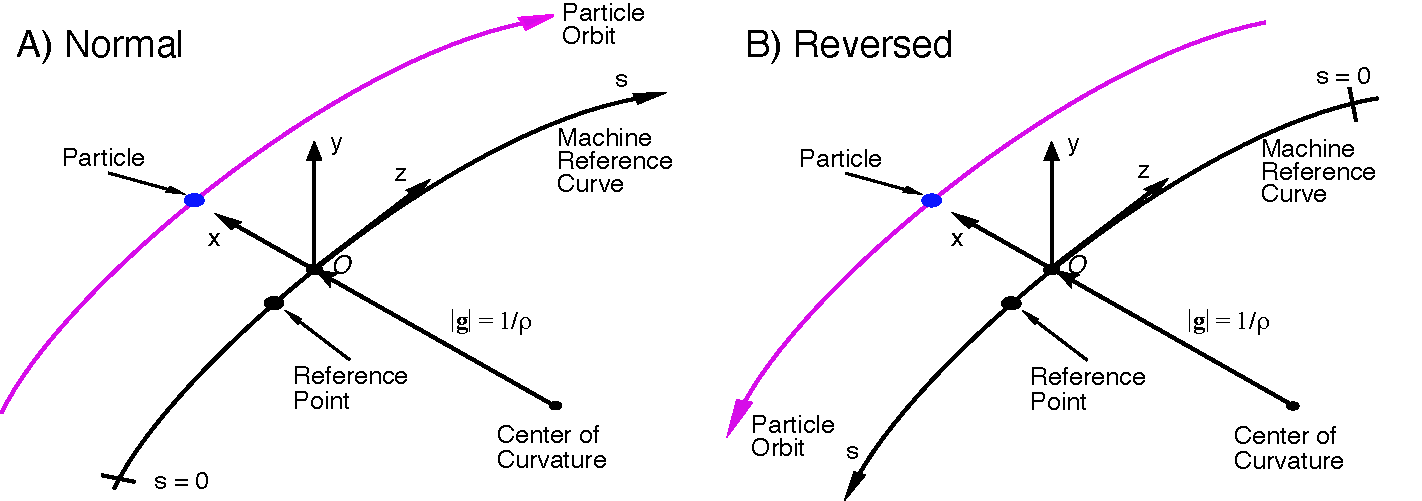
\includegraphics[width=6in]{machine-coords.pdf}
  \caption[Reference coordinate system.]
{The machine coordinate system. By construction, a particle's $z$ coordinate is zero.  This
is not to be confused with the phase space $z$ coordinate (\sref{s:phase.space}). The curvature
vector $\bfg$ lies in the $x$-$y$ plane and has a magnitude of $1/\rho$ where $\rho$ is the bending
radius. A) The $z$-axis will normally be parallel to the $s$-axis. B) For \vn{reversed} elements it
will be antiparallel. In both cases, the particle and reference particle are traveling in the
direction of greater $s$.}
  \label{f:machine.coords}
\end{figure}

The \vn{machine} coordinate system is the curvilinear coordinate system used for describing
a particle's position as shown in \fig{f:coords} and \fig{f:machine.coords}. 
The machine coordinate system is also used for
orientating lattice elements in space. At a given time $t$, a particle's position can be described
by a point $\calO$ on the reference orbit a distance $s$ relative to the reference orbit's zero
position plus a transverse $(x,y)$ offset. The point $\calO$ on the reference orbit is used as the
origin of the machine $(x, y, z)$ coordinate system with the $z$--axis tangent to the reference
orbit. The $z$--axis will generally be pointing in the direction of increasing $s$
(\fig{f:machine.coords}A) but, as discussed below, will point counter to $s$ for elements that are
longitudinally \vn{reversed} in orientation (\fig{f:machine.coords}B). 
The $x$ and $y$--axes are perpendicular to the reference
orbit and, by construction, the particle is always at $z = 0$. The coordinate system so constructed
is called the \vn{``machine coordinate system''} when there is need to distinguish it from the 
\vn{``element body coordinate system''}
(\sref{s:coords}) which is attached to the physical element. There is a separate reference orbit
for each branch (\sref{s:branch.def}) of a lattice.

\index{x_offset}\index{y_offset}
\index{x_rot}\index{y_rot}\index{wiggler}
The reference orbit may not correspond to the orbit that any actual particle could travel.
A common example is the \vn{wiggler} element where particles always oscillate about the reference
orbit which is a straight line.

Do not confuse this reference orbit (which defines the machine coordinate system) with the reference
orbit about which the transfer maps are calculated (\sref{s:twiss}). The former is fixed by the
lattice while the latter can be any arbitrary orbit.
